\part{APÉNDICES}

%%%%%%%%%%%%%%%%%%%%%%%%%%%%%%%%%%%%%%%%%%%%%%

\chapter{Tabla de símbolos matemáticos más frecuentes}

\begin{comment}




\end{comment}



\begin{table}[H]
\centering
\footnotesize
\begin{tabular}{|c|c|c|c|c|c|}
\multicolumn{1}{l}{$\qquad$} & \multicolumn{1}{l}{$\qquad$} & \multicolumn{1}{l}{$\qquad$} & \multicolumn{1}{l}{$\qquad$} & \multicolumn{1}{l}{$\qquad$} & \multicolumn{1}{l}{$\qquad$} \\ 
\hline
$\pm$ & $\mp$ & $>$ & $<$ & $\geq$ & $\leq$ \\
más menos & menos más & mayor & menor & mayor o igual & menor o igual \\ \hline
$\equiv$  & $\neq$ & $\approx$ & $\sim$ & $\propto$ & $\sum$ \\
idéntico/a & distinto/a & aproximado/a & similar & proporcional & sumatorio \\ \hline
$\prod$ & $\Delta$ & $\infty$ & $\emptyset$ & $\in$ & $\notin$ \\
productorio & incremento & infinito & vacío & pertenece & no pertenece \\ \hline
$\subset$ & $\subset$ & $\cup$ & $\cap$ & $\vee$ & $\wedge$  \\
contenido/a en & contiene a & unión & intersección & o (disyunción)  & y (conjunción) \\ \hline
$\parallel$ & $\nparallel$ & $\perp$ & $\not\perp$ & $\measuredangle$  & $\Rightarrow$ \\
paralelo/a & no paralelo/a & perpendicular & no perpendicular & ángulo & entonces \\ \hline
 $\Leftrightarrow$ & $\therefore$  & $\forall$ & $\exists$ & $\exists !$ & $\nexists$ \\
si y solo si & por tanto & para todo/a & existe al menos un/a & existe un/a único/a & no existe \\ \hline
 $\mathbb{N}$ &  $\mathbb{Z}$ &  $\mathbb{Q}$ &  $\mathbb{R}$ &  $\mathbb{R\sim Q}$ &  $\mathbb{C}$ \\
Naturales & Enteros & Racionales & Reales & Irracionales & Complejos \\ \hline

\end{tabular}
\end{table}
%%%%%%%%%%%%%%%%%%%%%%%%%%%%%%%%%%%%%%%%%%%%%%%%%%%%%%%%%%%%%%%%%






%%%%%%%%%%%%%%%%%%%%%%%%%%%%%%%%%%%%%%%%%%%%%%%%%%
\chapter{El método de inducción}
\label{inducción}

		
		El \emph{Principio de inducción matemática} es un método de demostración que se usa para probar que ciertas propiedades matemáticas se verifican para todo número natural. Por ejemplo:
		
		$1^2+2^2+3^2+...+n^2=\frac 1 6 n (n+1)(2n+1)$
		
		Podemos comprobar fácilmente que se cumple esta relación para los valores $n$ concretos que se nos ocurra, pero queremos \emph{demostrar} que la relación es válida $\forall n\in \mathbb N$ y para ello usaremos el \emph{Principio de inducción matemática}, que podemos considerar como un axioma y lo entenderemos as:
		
		\begin{axio}[Principio de inducción matemática] Queremos probar que la propiedad $P(n)$ se verifica $\forall n\in \mathbb N$. Tendremos que seguir dos pasos:
		
			
			1.-  Comprobaremos que el número 1 cumple la propiedad, es decir, $P(1)$ es cierta.
				
			2.- Comprobaremos que si un número $n$ cumple la propiedad, \emph{entonces} también la satisface el número $n+1$. Es decir, si comprobamos que $P(n)$ es cierta, \emph{entonces} también lo es $P(n+1)$
			
			
			"Si tengo una escalera infinita y quiero poder llegar a cualquier peldaño, necesito dos cosas: un primer escalón y saber cómo dar un paso"
		\end{axio}

		
		\begin{ejem} \label{sum-cuad-induc}
		Probar que $\forall n\in \mathbb N$, se cumple:
		$1^2+2^2+3^2+...+n^2=\frac 1 6 n (n+1)(2n+1)$	
		\end{ejem}
		 Evidentemente, para $n=1$ se cumple: $1=1$
		
		\begin{proof}[Apliquemos el método de inducción.]
			
		Supongamos ahora que la propiedad es cierta para $n$, hemos de conseguir demostrar que también lo ha de ser para $n+1$, es decir, se ha de cumplir la propiedad cambiando la $n$ por $n+1$:
		
		$1^2+2^2+3^2+...+n^2+(n+1)^2=\frac 1 6 (n+1) (n+2)(2(n+1)+1)$ (*)
		
		Vamos a por ello, sumemos $(n+1)^2$ a ambos lados de la ecuación que suponemos válida para $n$:
		
		
		$1^2+2^2+3^2+...+n^2\; \; +(n+1)^2=\frac 1 6 n (n+1)(2n+1)\; \; +(n+1)^2=$
		(sacando $n+1$ factor común:)
		$=(n+1) \left( \frac 1 6 n (2n+1) +(n+1) \right)=$
		
		$=(n+1)\frac 1 6 \left(  n (2n+1) + 6(n+1) \right)=$
		$\frac 1 6 (n+1) (2n^2+7n+6)=$
		
		$=\frac 1 6 (n+1) (n+2) (2n+3)\; $ que es la expresión (*) que queramos demostrar.%$\Box$
		\end{proof}
		
		 
		Es necesario subrayar la importancia de la demostración de las dos partes del principio de inducción. Veamos un ejemplo de la importancia de la primera parte:
		
		\begin{ejem}
			Todo número natural es igual al número natural siguiente.
		\end{ejem}
		
		\begin{proof}[Mala aplicación del principio de inducción.]
			
		Aplicando la parte 2 del principio de inducción, resulta que si esto es cierto para $n$, es decir, $n=n+1$, basta con sumar $1$ a cada parte de la igualdad y escribir $n+1=n+1+1=n+2$, también será cierto para $n+1$.
		
		Obviamente la demostración no está acabada y el teorema es falso, pues falta comprobar la primera parte del método de inducción: la propiedad se cumple para $n=1$: falso, $1\neq 2$ %$\qquad \qquad \qquad \qquad \Box$
		\end{proof}
		
		Vamos a ver unos ejemplos a continuación que nos convenzan de la importancia de no quedarse con una conjetura encontrada sino que hay que demostrarla siempre.
		
		\begin{ejem}
			Sea $p(x)=x^4+x+41$, trinomio estudiado ya por Euler. Se tiene que $p(0)=41$, primo; $p(1)=43$, primo, y hasta $x=10$ se obtienen los números 47, 53, 61, 71, 83, 97, 113, 131 y 151 respectivamente, todos primos. Estaríamos tentados a afirmar que en este trinomio, al sustituir $x$ por cualquier número natural se obtiene un número primo, pero no es así, ya que, p.e., para $x=40$ tenemos $p(40)=40^2+40+41=40(40+1)+41=40\cdot 41+41=(40+1)\cdot 41=41^2$, que evidentemente no es un número primo.
		\end{ejem}
		
		 \begin{ejem} Consideremos los números de la forma $N(n)=2^{2^n}+1$. Para $n=0,1,2,3,4$ se obtienen $3, 5, 17, 257, 65537$, que son números primos. Fermat (s.XVII) aceptaba que todos los números obtenidos por esta fórmula eran primos. Fue Euler (s. XVIII) encontró $N(5)=4294967297=641\cdot 6700417$, compuesto.
		\end{ejem}
		
		\begin{ejem}
 			Leibniz (s. XVII) demostró que para cualquier número natural $n$, el número $n^3-n$ es siempre divisible por $3$, el número $n^5-n$ divisible por $5$, $n^7-n$ divisible por $7$. De ahí, supuso que si $k$ era un número natural impar, $n^k-n$ seria divisible por $k$, pero pronto observó que $2^9-2=510$ que no es divisible por $9$.
 		\end{ejem}
 		
 	    \begin{ejem}
 			$F(n)=991n^2+1$ no da nunca un cuadrado perfecto para $n=1,2,3,...$, por muchos das o años que nos dediquemos a ello. En efecto, el primer número natural para el que $F(n)$ resulta un cuadrado perfecto es:
 			
 			$n=12055735790331359447442538767.$
 		\end{ejem}
 		
 		 Con estos ejemplos podemos llegar a una sencilla pero importante conclusión: una conjetura puede ser cierta en muchos casos particulares pero si no hay demostración, nunca será un teorema.
 		 
 		 
\vspace{1cm}

\begin{miejercicio}

En el tema \ref{complejos}, `Números Complejos', intuimos la fórmula para	la potenciación: 

$ \quad \boldsymbol{ (r_\alpha)^n\ = \ r^n_{	\ n\alpha} }\, , \quad $ demostremos ahora que es cierta.

\vspace{2mm} \photon \photon \photon \photon \photon \photon \photon \photon \photon \photon \photon \photon \photon 

\vspace{2mm} $\triangleright\quad$ ?`Es certa la fórmula para $n=1\, $ ? $\quad (r_\alpha)^1=r_\alpha\, , \ $ evidentemente.

\vspace{2mm} $\triangleright\quad$ Suponiendo que la fórmula es cierta para $n-1,\ $ es decir, $\ (r_\alpha)^{n-1} \ = \ r^{n-1}_{\quad (n-1)\alpha}\, , \ $ ?`lo será para $\ n\, $?

\vspace{2mm} $(r_\alpha)^n= (r_\alpha)^{n-1} \cdot r_\alpha=(r^{n-1} \cdot r)_{\ (n-1)\alpha+\alpha}=r^n_{\ n\alpha} $ \QED

\vspace{2mm} Queda demostrado por inducción que la fórmula es válida $\ \forall n\in \mathbb N$
\end{miejercicio}

 
 %%%%%%%%%%%%%%%%%%%%%%%%%%%%%
 
 
 
 

%%%%%%%%%%%%%%%%%%%%%%%%%%%%%%%%%%%%%%%%%%%%%%%%%%%%%%%%%%%%%%%%%%%%%%%%%%
%%%%%%%%%%%%%%%%%%%%%%%%%%%%%%%%%%%%%%%%%%%%%%

\chapter{Puntos Mágicos}\label{puntosmagicos}

Problema+ del capítulo \ref{recta}, ``La recta en el plano''.

\vspace{5mm}

\textbf{\emph{Puntos Mágicos}}
\vspace{5mm}
\begin{destacado} 
\begin{adjustwidth}{20pt}{20pt}
\vspace{2mm}
\color{NavyBlue}
\vspace{2mm} \textbf{\emph{En un vetusto documento, se hallaron las siguientes instrucciones: Partiendo de la intersección del Camino del Rey con el Camino de la Reina, sígase hacia el Norte por el primero y búsquese un pino y después un arce. Regrésese a la intersección. Hacia el Oeste, por el Camino de la Reina, hay un olmo y hacia el Este, en ese mismo camino, hay un abeto. El punto en el cual la recta determinada por el olmo y el pino corta a la recta determinada por el arce y el abeto es uno de los dos puntos mágicos. El otro punto mágico es la intersección de la recta determinada por el abeto y el pino con la recta determinada por el olmo y el arce. El tesoro está enterrado donde la recta que une los dos puntos mágicos corta al Camino de la Reina.}}

\vspace{2mm} \textbf{\emph{Enseguida se comenta que una patrulla halló el olmo a 4 km, el abeto a 2 km y el pino a 3 km (todas estas distancias medidas a partir de la intersección). Del arce ... ninguna traza.}}

\vspace{2mm} \textbf{\emph{No obstante, mediante las indicaciones, la patrulla logró hallar el tesoro. ?`Cómo fue esto posible? Uno de los patrulleros habló de cuán afortunados habían sido por haber encontrado el pino. El jefe de la patrulla sonrió y dijo: ``Tampoco necesitábamos el pino''. !`Demostremos que estaba en lo cierto! }}
\color{Black}
\vspace{2mm}
\end{adjustwidth}
\end{destacado}

\vspace{4mm} \begin{flushright} \emph{ ``Magia y encanto de la Matemática''. Jesús Alfonso Pérez Sanchez. } \end{flushright}

\begin{flushright}
\textsf{Se incluye, en el repositorio, un applet del problema creado con Geogebra.}	
\end{flushright}



\vspace{5mm}
\color{gris}
\underline{Ayuda}
\begin{itemize}
\item Supón, en un principio que el arce está a 5 km.
\item Supón, ahora que no conocemos la posición del arce, que esté a $p$ km por ejemplo.
\item Supón, finalmente, que tampoco conocemos la posición del pino, que esté a $q$ km.
\item Deberás poder encontrar que la posición del Tesoro es independiente de $p$ y $q$.	
\end{itemize}
\color{black}

\begin{figure}[H]
	\centering
	\includegraphics[width=1\textwidth]{img-ga/puntosmagicos.png}
\end{figure}

$Olmo(-4,0),\ \ Abeto(2,0),\ \ Pino(0,p),\ \ Arce(0,q);\ \  camino Reina: \ y=0;\ \ camino Rey:\ x=0$

$r_{OlPi} \, \cap \, r_{AbAr} \ = \ M_1;\quad r_{OlAr}\, \cap \, r_{AbPi} \ = \ M_2 \quad \Rightarrow \quad r_{M_1M_2} \, \cap \ camino Reina \ = \ Tesoro$


\vspace{10mm} 

\textcolor{red}{$\boxed{\ M_1 \ }$}

$r_{OlPi}:\ \begin{cases} \ Ol(-4,0)\\ \ Pi(0,p)\end{cases} \equiv \begin{cases} \ Ol(-4,0)\\ \ \vec v_{OlPi}=(4,p) \ \to \ m_{OlPi}=\dfrac p 4 \end{cases}
 \quad \ \Rightarrow \ y=\dfrac p 4 \, (x+4)$
 
 $r_{AbAr}:\ \begin{cases} \ Ab(2,0)\\ \ Ar(0,q)\end{cases} \equiv \begin{cases} \ Ab(2,0)\\ \ \vec v_{AbAr}=(-2,q) \ \to \ m_{AbAr}=-\dfrac q 2 \end{cases}
 \ \Rightarrow \ y=-\dfrac q 2 \, (x-2)$

$M_1=r_{OlPi}\, \cap \, r_{AbAr} \ \to \ \dfrac p 4 x+p=-\dfrac q 2 x+q \ \to \ \left(\dfrac p4+\dfrac q2 \right)\, x=\dfrac{2q+p}{4}\, x= q-p  \ \to \ x=\dfrac{4(q-p)}{2q+p}$

$y=\dfrac p 4 (x+4)=\dfrac p 4 \left[ \dfrac{4(q-p)}{2q+p}+4\right]=p\, \dfrac{q-p}{2q+p}+p=\dfrac{p(q-p)+p(2q+p)}{2q+p}=\dfrac{3qp}{2q+p}$

$$ \text{Luego, } \qquad \boldsymbol{ M_1 \ = \ \left( \, \dfrac{4(q-p)}{2q+p}\, , \, \dfrac{3qp}{2q+p} \, \right) } $$



\vspace{5mm} \textcolor{red}{$\boxed{\ M_2 \, \cap \, caminoReina\ }$}

$r_{OlAr}:\, \begin{cases} \ Ol(-4,0) \\ \ Ar(0,q) \end{cases} \equiv \begin{cases} \ Ol(-4,0)\\ \ \vec v_{OlAr}=(4,q) \ \to \ m_{OlAr}=\dfrac{q}{4} \end{cases} \quad  \Rightarrow \ y=\dfrac q 4 \, (x+4)$

$r_{AbPi}:\, \begin{cases} \ Ab(2,0) \\ \ Pi(0,p) \end{cases} \equiv \begin{cases} \ Ab(2,0)\\ \ \vec v_{AbPi}=(-2,p) \ \to \ m_{AbPi}=-\dfrac{p}{2} \end{cases} \ \Rightarrow \ y=-\dfrac p 2 \, (x-2)$

$M_2 = r_{OlAr} \, \cap \, r_{AbPi} \ \to \ 
\dfrac q 4 x+q=-\dfrac p 2 x + p \ \to \ \left( \dfrac q 4 + \dfrac p 2 \right)\, x=\dfrac{q+2p}{4}\, x= p-q \ \to \ x=\dfrac{4(p-q)}{q+2p}$

$y=\dfrac q 4 (x+4)=\dfrac q 4 \left[\dfrac{4(p-q)}{q+2p} + 4 \right] = \dfrac{q(p-q)}{q+2p}+q=\dfrac{q[(p-q)+(q+2p)]}{q+2p}=\dfrac{3pq}{q+2p}$

$$\text{Luego, } \qquad \boldsymbol{ M_2 \ = \ \left( \, \dfrac{4(p-q)}{q+2p} º, , \, \dfrac{3pq}{q+2p} \, \right) } $$


\vspace{5mm} \textcolor{red}{$\boxed{\ r_{M_1M_2} \ }$}

$\overrightarrow{M_1M_2}\ = \ M_2-M_1$

--- Componente $x:\qquad \dfrac{4(p-q)}{2p+q}-\dfrac{4(q-p)}{p+2q}=
\dfrac{4(p-q)}{2p+q}+\dfrac{4(p-q)}{p+2q}=
4(p-q)\, \left[ \dfrac{1}{2p+q}+\dfrac{1)}{p+2q} \right]=
\dfrac{4(p-q)\, (3p+3q)}{(2p+q)(q+2p)}=
\dfrac{12(p^2-q^2)}{(2p+q)(2q+p)}$

--- Componente $y: \qquad \dfrac{3pq}{2p+q}-\dfrac{3pq}{p+2q}=\dfrac{3pq\, (p+2q-2p-q)}{(2p+q)(p+2q)}=\dfrac{3pq\, (q-p)}{(2p+q)(p+2q)}$

--- Pendiente: $\qquad  m \ = \ 
\dfrac {\dfrac{3pq\, (q-p)}{(2p+q)(p+2q)}} {\dfrac{12(p^2-q^2)}{(2p+q)(2q+p)}} =
\dfrac{3pq\, (q-p)}{12\, (p+q)\, (q-p)} \ = \ \dfrac{pq}{4(p+q)}$

--- Recta $M_1M_2:\qquad y-\dfrac{3pq}{p+2q} \ = \ \dfrac{pq}{4(p+q)}\, \left( \, x-\dfrac{4(p-q)}{p+2q}\, \right)$

\vspace{5mm} \textcolor{red}{$\boxed{\ Tesoro \ }$}

Tesoro $\, = r_{M_1M_2} \, \cap \, caminoReina \, (y=0)\ \ \to $ haciendo $y=0$ en la ecuación anterior,

$\dfrac{-3pq}{p+2q}=\dfrac{pq}{4(p+q)} x -\dfrac{4pq(p-q)}{4(p+q)(p+2q)} \ \to \ 
\dfrac{pq}{4(p+q)} x=\dfrac{3pq(p+q)}{(p+q)(p+2q)}-\dfrac{pq(p-q)}{(p+q)(p+2q)} \ \to \ $

$\to \ x=\dfrac{4(p+q)}{pq}\, \dfrac{pq}{(p+q)(p+2q)}\, \left[ 3(p+q)+p-q  \right]\dfrac{4}{p+2q}\, [2(p+2q)] \ \Rightarrow \ \boldsymbol{ \boxed{ \ x \ = \ 8 \ } }$


\vspace{5mm}\textsf{El tesoro se encuentra en el camino de la Reina a $8$ km hacia el Este desde el origen, con independencia de donde se encuentren tanto el Arce como el Pino} \textcolor{gris}{$\quad (x=8\, ; \ \ \ \forall p\, , \ \forall q)$}


%%%%%%%%%%%%%%%%%%%%%%%%%%

\chapter{Cuadrado inscrito en triángulo}\label{cuadradoentriangulo}

\vspace{10mm}

Una posible idea para abordar el problema sería:

\begin{figure}[H]
	\centering
	\includegraphics[width=1\textwidth]{img-ga/cuadradoentriangulo.png}
\end{figure}

Siempre podemos situar nistro triángulo con un vértice en el origen ($A$) y una lado ($AB$) en el eje $OX$. Conocido el triángulo conocemos la ecuación del lado $AC \ \to \ y=m\, x \, ; \ \ m=\tan A$

Disponemos cuadrados en el interior del triángulo con bases en el lado $AB$ y alturas hacia la recta $AC$, como se observa en la figura.

$r_{PQ}:\, \begin{cases} \ P(x_1+mx_1,mx_1) \\ \ Q(x_2+mx_2,mx_2) \end{cases} \to \ m=\dfrac{mx_2-mx_1}{x_2+mx_2-x_1-mx_1}=\dfrac{m(x_2-x_1)}{(x_2-x_1)(1+m)}=\dfrac{m}{1+m}$

$r_{PQ}:\, \begin{cases} \ P(x_1+mx_1,mx_1) \\ \ m=\dfrac{m}{1+m} \end{cases} \ \to \ y-mx_1=\dfrac{m}{1+m}(x-x_1-mx_1)=\dfrac{m}{1+m}[x-(1+m)x_1] $

$r_{PQ}:\ \ \boldsymbol{ y} \ =\dfrac{m}{1+m}\, x- 
\dfrac{\cancel{(1+m)}\,\bcancel{ mx_1} }{\cancel{(1+m)}} 
+ \bcancel{mx_1}
=\ \boldsymbol{ \dfrac{m}{1+m}\, x}$

\vspace{5mm} Hemos obtenido $r$  independiente de  $x_1$  y de $x_2$

La intersección de  $r_{PQ}$ con la recta que pasa por $BC$ nos proporcionará el vértice BUSCADO para que, proyectando verticalmente sobre el lado $AB$ y horizontalmente sobre $AC$ y, esta última proyección, vuelta a proyectar verticalmente sobre $AB$, nos den los 4 vértices del cuadrado que está insertado en el triángulo.



AMPLIACIÓN:   Como  $m=tan A$   y   $m_{PQ}=\tan \theta$ ,   buscar la relación entre  $A$  y  $\theta$ (La recta $BC$ tiene por pendiente  $m_{BC}=\ tan(C)<0$ )



%%%%%%%%%%%%%%%%%%%%%%%%%%%%%%%%%%%%%%%%%%%%%%%%%%%%%%%%%%%%%%%%%



\chapter{Bola que rebota}\label{simetricos}

Problema $\boldsymbol{+}$, Tema 11 `La recta en el plano'

\vspace{10mm}

\begin{figure}[H]
	\centering
	\includegraphics[width=1\textwidth]{img-ga/simetricos.png}
\end{figure}

\vspace{5mm}

$B'$ es el simétrico de $B$ respecto de $s$; $B''$ es el simétrico de $B'$ respecto de $r$.

$C$ es el punto de intersección de la recta $r_{AB''}$ con la recta $r$ y $D$ es el punto de intersección de la recta $r_{CB'}$ con la recta $s$.

\emph{El trayecto más corto es el $\boldsymbol{ \ A \ \to \ C \ \to D \ \to \ B }$}



\chapter{Ecuación general de una cónica} \label{fcuadraticas}


Una cónica viene descrita por una forma general cuadrática como $\ Ax^2+Bxy+Cy^2+Dx+Ey+F=0$. La presencia del término cruzado en $xy$  dificulta el clasificarla y determinar cuales son sus elementos (en física se llama a estos casos \emph{`variables acopladas'} y complican enormemente la solución de los problemas en que aparecen). 

En este apéndice se verá una que una forma de eliminar estos términos cruzados de la cónica consiste en aplicar un giro determinado de los ejes coordenados respecto al origen, pasando de unos ejes $x$-$y$ a unos nuevos $X$-$Y$, girados un ángulo $\phi$ respecto al origen de coordenadas.

\section{Rotación de ejes}


\begin{multicols}{2}
Un mismo punto $P$ del plano se escribirá como $P(x,y)$ en el sistema de ejes $x$-$y$ y como $P(X,Y)$ en la referncia $X$-$y$. Veamos como pasar de unas a otras coordenadas.

\vspace{2mm} $r$ distancia de $P$ al origen.

\vspace{1mm} $\phi$ ángulo de rotación de los ejes.

\vspace{1mm} $\theta$ ángulo que forma $r=OP$ con el eje $x$ inicial.

\vspace{1mm} De la figura se puede observar que:

\begin{figure}[H]
	\centering
	\includegraphics[width=.5\textwidth]{img-conicas/conicas50.png}
	\end{figure}		
\end{multicols}

$$ \left. \begin{array}{lcl}
 X&=&r\cos \, \theta \\ Y&=&r\sin \, \theta	
 \end{array} \qquad  \right|
  \qquad 
 \begin{array}{lcl}
 x&=&r\cos \, (\theta+\phi) \\ y&=&r\sin \, (\theta+\phi)	
 \end{array}$$

Usando fórmulas del seno y coseno de la suma de ángulos aprendidas en el tema de `fórmulas trigonometricas',

$x=r\cos(\theta+\phi)=r(\cos \theta \cos \phi-\sin \theta \sin \phi)=(r\cos \theta)\cos \phi-(r\sin \theta)\sin \phi=X\cos \phi-Y\sin \phi$

$y=r\sin(\theta+\phi)=r(\sin \theta \cos \phi+\cos \theta \sin \phi)=(r\sin \theta)\cos \phi+(r\cos \theta)\sin \phi=X\sin \phi+Y\cos \phi$

Estas dos relaciones sirven pasa pasar del sistema $X$-$Y$ al $x$-$y$. Despejando $X$ e $Y$ de este sistema se llega a las ecuaciones para el cambio inverso. Resumiendo ambos cambios de sistema de referencia, obtenemos:

$$\boldsymbol{ \boxed{ \ \ 
\left. 
\begin{array}{lcl}
\\ x&=&X\cos \phi-Y\sin \phi \\ \\ y&=&X\sin \phi+Y\cos \phi \\ \, \end{array} \qquad \right| \qquad 
\begin{array}{lcr} \, \\ X&=& x\cos \phi+y\sin \phi \\ \\ Y&=&-x\sin \phi+y\cos \phi \\ \,  \end{array} \ \ } }$$

\vspace{10mm} \underline{Ejemplo:}

Sea $P(2,-4)$ un punto expresado en un sistema de referencia ortonormal $x$-$y$ sobre el que aplicamos un giro de $30^o$ a los ejes respecto del origen de coordenadas. ?`Cuáles son las nuevas coordenadas de $P$ en el nuevo sistema de referencia $X$-$Y$?

\rule{200pt}{0.1pt}

$\left.
\begin{array}{lcrrr}  X&=& x\cos \phi+y\sin \phi &= \ 2\cos 30+(-4)\sin 30&=\quad \sqrt{3}-2
\\  Y&=&-x\sin \phi+y\cos \phi &=-2\sin 30 +(-4)\cos 30&=-1-2\sqrt{3}  \end{array} \quad \right\} \ \ \to $

$\to \quad  P_{x\text{-}y}(2,-4) \ \equiv \ P_{X\text{-}Y} \big(\sqrt{3}-2 \, , \, -1-2\sqrt{3} \big)$


\vspace{5mm}
\vspace{2mm} \underline{Ejercicio}: $\quad$ Demostrar que al girar $45^o$ la ecuación $xy=1$ se obtiene una hipérbola equilátera \textcolor{gris}{($a=b$)} y determinar sus elementos.


\rule{200pt}{0.1pt}


\begin{multicols}{2}

$\left. \begin{array}{lclcl}
x&=&X\cos \phi-Y\sin \phi&=&\dfrac{X}{\sqrt{2}}-\dfrac{Y}{\sqrt{2}} \\ y&=&X\sin \phi+Y\cos \phi&=& \dfrac{X}{\sqrt{2}}+\dfrac{Y}{\sqrt{2}} \end{array}   \right\} \ \to$

\vspace{2mm} $\to \quad $ sustituyendo en $x\cdot y=1 \quad \Rightarrow$

\vspace{2mm} $ \left( \dfrac{X}{\sqrt{2}}-\dfrac{Y}{\sqrt{2}} \right) \cdot \left( \dfrac{X}{\sqrt{2}}+\dfrac{Y}{\sqrt{2}} \right) \ = \ \boldsymbol{ \dfrac{X^2}{2}-\dfrac{Y^2}{2} = 1 }$


\vspace{4mm} $\dfrac{X^2}{2}-\dfrac{Y^2}{2} = 1 \ $ es la ecuación de una hipérbola equilátera con $a=b=\sqrt{2}$ y $c=\sqrt{a^2+b^2}=2$, luego $\varepsilon = 2/\sqrt{2}=\sqrt{2}$

\vspace{2mm} Vértices en $(\pm \sqrt{2}, 0)$ y focos en $(\pm 2,0)$
\begin{figure}[H]
	\centering
	\includegraphics[width=.5\textwidth]{img-conicas/conicas51.png}
	\end{figure}		
\end{multicols}


\section{Ecuación general de una cónica}

Deseamos efectuar una rotación de ejes de ángulo $\phi$ de modo que la forma cuadrática que representa a la cónica, $\mathcal C:\ Ax^2+Bxy+Cy^2+Dx+Ey+F=0$, en los nuevos ejes rotados ($X$-$Y$) se expresen sin términos cruzados (que las nuevas variables estén desacopladas), así: $\ \mathcal C:\ A'X^2+C'Y^2+D'X+E'Y+F'=0$, es decir, tenemos que determinar cual es el valor de $\phi$ para que $B'=0$.


Teniendo en cuenta las fórmulas vistas anteriormente para el cambio de sistema de referencia al rotar $\phi$ radianes los ejes, podremos escribir la forma cuadrática (cónica) en los ejes girados como:

$A(X\cos \phi-Y\sin \phi)^2+B(X\cos \phi-Y\sin \phi)(X\sin \phi+Y\cos \phi)+C(X\sin \phi+Y\cos \phi)^2+D(X\cos \phi-Y\sin \phi)+E(X\sin \phi+Y\cos \phi)+F=0$

Expandiendo y comparando con $\ C:\ A'X^2+C'Y^2+D'X+E'Y+F'=0$:

\vspace{5mm}
\begin{center}
$\begin{array}{lcl}
	A'&=&A\cos^2 \phi+B\sin \phi \cos \phi + C\sin^2 \phi \\
	B'&=&2(C-A)\sin \phi \cos \phi +B (\cos^2 \phi-\sin^2 \phi) \\
	C'&=&A\sin^2 \phi-B\sin \phi \cos \phi + C\cos^2 \phi \\
	D'&=&D\cos \phi+E\sin \phi \\
	E'&=&-D\sin \phi+E\cos \phi \\
	F'&=&F
 \end{array}$	
\end{center}
\vspace{5mm}

$B'=0 \ \ \Rightarrow \ \ 2(C-A)\sin \phi \cos \phi +B (\cos^2 \phi-\sin^2 \phi)=0 \ \ \to \  (C-A)\sin 2\phi
+B\cos 2\phi=0 \ \ \Rightarrow  $


$$\Rightarrow \qquad \boxed{ \ \boldsymbol{ \tan 2\phi \ = \ \dfrac{B}{A-C}} \ }$$


Ángulo a rotar para que la cónica sea de variables separadas, no tenga términos cruzados o se exprese con variables desacopladas, para que no hayan términos cruzados $xy$.

\vspace{10mm} \underline{Ejemplo}: $\quad$ Establecer una rotación de ejes para que la ecuación $\ 6\sqrt{3}\, x^2+6\, xy+4	\sqrt{3}\, y^2=12\sqrt{3}\ $ no tenga términos cruzados. Clasificar la cónica y determinar sus elementos.

\rule{250pt}{0.1pt}

$\tan 2\phi=\dfrac{B}{C-A}=\dfrac{6}{6\sqrt{3}-4\sqrt{3}}=\dfrac{6}{2\sqrt{3}}=\dfrac{3}{\sqrt{3}}=\sqrt{3}\quad \to \quad 2\phi=60^o \quad \Rightarrow \quad \phi=30^o$ 

Cambios: $\quad \left\{ \  \begin{array}{lclcl}
 x&=&X\cos 30-Y\sin 30&=&\dfrac{\sqrt{3}\, X}{2}-\dfrac{Y}{2} \\
 y&=&X\cos 30+Y\sin 30&=&\dfrac{X}{2}+	\dfrac{\sqrt{3}\, X}{2}
 \end{array} \right. \, , \  $  luego
 
 $6\sqrt{3} \left( \dfrac{\sqrt{3}\, X}{2} - \dfrac Y 2 \right)^2 +
 6 \left( \dfrac{\sqrt{3}\, X}{2} - \dfrac Y 2 \right) \left(\dfrac X 2 + \dfrac{\sqrt{3}\, Y}{2}  \right) + 4\sqrt{3} \left(\dfrac X 2 + \dfrac{\sqrt{3}\, Y}{2}  \right)^2 \ = \ 21\sqrt{3}$


desarrollando, $\ 7\sqrt{3}\, X^2 +3\sqrt{3}\, Y^2 = 21 \sqrt{3} \, , \  $ dividiendo por $\ 21 \sqrt{3}\, , \quad $
$\boldsymbol{ \dfrac {X^2}{3} \ + \ \dfrac{Y^2}{7} \ = \ 1 } \quad $ 

Se trata de una elipse vertical centrada en el origen con semiejes $a=7$ y $b=3$, por lo que \textcolor{gris}{$(a^2=b^2+c^2)$} $\ c=\sqrt{40}$ y $\varepsilon = \sqrt{40}/7\approx 0.90<1$, que está \emph{girada un ángulo de $30^o$}

\begin{figure}[H]
	\centering
	\includegraphics[width=.5\textwidth]{img-conicas/conicas52.png}
	\end{figure}


\vspace{10mm} \underline{Observaciones}:

No es siempre tan sencillo el cálculo de $\phi$. En muchas ocasiones serán de utilidad las fórmulas aprendidas de las razones trigonométricas del ángulo mitad:

$$ \cos \phi \ = \ \sqrt{\dfrac{1+\cos 2\phi}{2}} \qquad \qquad  \sin \phi \ = \ \sqrt{\dfrac{1-\cos 2\phi}{2}} $$


\vspace{10mm} \underline{Ejercicio}: $\quad 64x^2+96xy+36y^2-15x+20y-25=0$ 

\vspace{5mm}
\begin{multicols}{2}
$\cos \phi=\sqrt{\dfrac{1+7/25}{2}}=\dfrac 4 5$

$\sin \phi=\sqrt{\dfrac{1-7/25}{2}}=\dfrac 3 5$
\begin{figure}[H]
	\centering
	\includegraphics[width=.2\textwidth]{img-conicas/conicas53.png}
	\end{figure}	
\end{multicols}

Cambio: $ \quad \left\{ \ \begin{array}{lcl} x&=&\dfrac 4 5 X - \dfrac 3 5 Y \\  \\ y&=& \dfrac 3 5 X + \dfrac 4 5 Y \end{array} \right. \quad $ sustituyendo,


\begin{small}
$64 \left( \dfrac 4 5 X - \dfrac 3 5 Y  \right)^2+96\left( \dfrac 4 5 X - \dfrac 3 5 Y  \right)\left( \dfrac 3 5 X + \dfrac 4 5 Y  \right)+36 \left( \dfrac 3 5 X + \dfrac 4 5 Y  \right)^2-15 \left( \dfrac 4 5 X - \dfrac 3 5 Y  \right) +20 \left( \dfrac 3 5 X + \dfrac 4 5 Y  \right)-25=0$
\end{small}

desarrollando, $\quad 100X^2+25Y-25=0 \quad \Rightarrow \quad \boldsymbol{X^2 \ = \ - \dfrac 1 4 \, (Y-1)}$

Ecuación que representa a una parábola hacia la izquierda, desplazada al punto $(0,1)$ (en la referencia $X$-$Y$) y girada un ángulo de $\phi=atan \dfrac {24}{7}\approx 37^o$.

Comparando con $X=-4pY \ \to \ 4p=1/4 \ \to \ p=1/16$. El foco está $1/16$ a la izquierda del origen, $F(0,1-1/16)=(0,15/16)$ y la directriz está a $1/16$ a la derecha del origen, $Y=1+1/16=17/16$.

\begin{figure}[H]
	\centering
	\includegraphics[width=.5\textwidth]{img-conicas/conicas54.png}
	\end{figure}


\vspace{15mm} 
\section{Discriminante de una cónica}

\begin{tikzpicture}
	\fill [left color=red!50, right color=teal!50] (0,0) rectangle (3.5,.1);
	\fill [left color=teal!50, right color=blue!50] (3.5,0) rectangle (7.5,.1);
	\end{tikzpicture}
\vspace{1cm}


\begin{cuadro-naranja}
	$$\boxed{ \ Ax^2+Bxy+Cy^2+Dx+Ey+F=0 \quad \to \quad \boldsymbol{\Delta=B^2-4AC} \quad \Rightarrow \quad \begin{cases} \ \Delta <0 & \to \text{ Elipse} \\ \ \Delta=0 &\to \text{ Parábola} \\ \ \Delta>0 &\to \text{ Hipérbola} \end{cases} \ }$$
	\vspace{1mm}
\end{cuadro-naranja}

Si se aplica una rotación cualquiera $\phi$ de ejes, la cónica se transforma en 

$ A'x'^2+B'x'y'+C'y'^2+D'x'+È'y'+F'=0  \ \to \ \Delta'=B'-4A'C' $

Se puede demostrar que, $\forall \phi: \quad \Delta=\Delta'$

En lenguaje físico podemos decir que el discriminante es un invariante (no cambia) bajo la rotación de ejes, se conserva (\emph{el discriminante es invariante bajo rotación}).

Si elegimos el cambio adecuado para desacoplar las variables (que desaparezcan los términos curados, en $xy$), tendremos que:

Para $\ \phi \ \big/ \ B'=0 \ \Rightarrow \ \Delta  \ = \ -4A'C' \ = \ B^2-4AC$

Tendremos: $\qquad \left\{ \ \  \begin{array}{lclcl} \ \Delta < 0 &\to& \ A'C'>0 \text{ mismo signo } &\to& \ \text{Elipse} \\ \ \Delta=0 &\to& \ A'=0 \ \vee \ C'=0  &\to& \ \text{Parábola} \\ \ \Delta>0 &\to& \ A'C'<0 \text{ distinto signo }  &\to& \ \text{Hipérbola} \end{array} \right.$ \QED
 	

\vspace{20mm}

\textcolor{NavyBlue}{\emph{Una descripción geométrica unificada de cónicas se obtiene cuando se usan coordenadas polares}.}



\begin{comment}

%%%%%%%%%%%%%%%%%%%%%%%%%%%%%%%%%%%. SECCIONES
\chapter{texto}

\begin{tikzpicture}
	\fill [left color=red!50, right color=teal!50] (0,0) rectangle (6.5,.2);
	\fill [left color=teal!50, right color=blue!50] (6.5,0) rectangle (11.5,.2);
	\end{tikzpicture}

\vspace{1cm}
\section{texto}

\begin{tikzpicture}
	\fill [left color=red!50, right color=teal!50] (0,0) rectangle (3.5,.1);
	\fill [left color=teal!50, right color=blue!50] (3.5,0) rectangle (7.5,.1);
	\end{tikzpicture}
\vspace{0.5cm}

\subsection{texto}
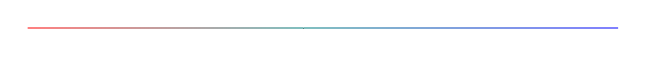
\begin{tikzpicture}
	\fill [left color=red!50, right color=teal!50] (0,0) rectangle (3.5,.01);
	\fill [left color=teal!50, right color=blue!50] (3.5,0) rectangle (7.5,.01);
	\end{tikzpicture}
\vspace{0.5cm}


%%%%%%%%%%%%%%%%%%%%%%%%%%%%%%%%%%%. \begin{ ------>. 
detsacado;  cuadro-naranja;  cuadro-gris;  miejercicio (solución extensa);  mipropuesto (solución corta y fuera del cuadro)

%%%%%%%%%%%%%%%%%%%%%%%%%%%%%%%%%%%. CURIOSIDAD
\vspace{1cm}
\color{ForestGreen!80}
\rule{250pt}{0.2pt}
Texto
\vspace{-8mm}
\begin{flushright}
\rule{250pt}{0.2pt}		
\end{flushright}	
\color{black}
\end{comment}
